\documentclass[11pt]{article}

\usepackage{fullpage}
\usepackage{url}
\usepackage{paralist}
\usepackage{graphicx}
\usepackage[small]{caption}
\usepackage{subfig}

% =========
\usepackage{color}

% The xxx tag is intended to denote urgent text that needs addressing.
% The meh tag is intended to highlight text that needs some loving or which
% we're not sure should make primetime
\newcommand{\xxx}[1]{{\bf \color{red} #1}}
\newcommand{\meh}[1]{{\bf \color{blue} #1}}

% =========

\title{\xxx{Linguistic Classification of Objects}}
\author{Rob Goeddel \and Lauren Hinkle \and James Kirk \and Aaron Mininger}
\date{}

\begin{document}
\maketitle

\begin{abstract}
\xxx{Abstract goes here, 1 par. max}
Dijkstra was a cool guy and it's fun to cite his papers~\cite{dijkstra1959}.
\end{abstract}

\section{Introduction}
\xxx{Problem description and motivation. Why do you want to solve this
    problem? What's the impact if you can solve this problem?}
Language is a powerful tool that is just coming into its own as the human
interface for various systems. Apple's Siri is an excellent example of this,
making interaction with your phone and web-search effectively seamless
compared to the tedious data entry required before.

Learning systems in AI can also benefit from greater understanding of
language. Take, for example, a robotic arm system with knowledge of only
several nouns and actions: dish, sink, grab/move object, and turning on/off
the sink, and the spatial concept of in. The robot can now be taught that
``washing the dishes'' means to put the dishes in the sink and turn on the
sink. Even though the robot has never seen anyone wash the dishes before, now
it should be able to wash dishes, itself, and even could learn the word
``wash'' and apply it to another object such as an apple. This is a powerful
and intuitive way for humans to interact with a system, one which it does not
take a computer scientist to understand.

Our goal is to train a system to know a small vocabulary of nouns, adjectives,
and actions. As a proof of concept, we want to be able to play the children's
game ``I spy'' with a robotic arm. The arm's ``eyes'' will be a Microsoft
Kinect (or, with some small probability, a stereo camera rig) capable of
returning RGB-D data for classification. Given this groundwork, such a system
should be straightforward to extend and train to recognize a more extensive
vocabulary, and thus can be taught more complex actions. It could be deployed
on robots in service tasks or in non-robotics systems where a verbal interface
offers improvements in efficiency, safety, etc. \xxx{Examples?}

\section{Proposed Method}
\xxx{How are you going to solve this problem? Why should the proposed method
    work? Provide technical details of your approach if you are proposing a
    novel method.}
To initially address this problem, we propose to learn our base vocabulary
under supervised learning with data hand-labeled to denote words applying to
the supplied objects. Classification will be performed on a feature vector
derived from the RGB-D data sticking to features dealing with shape, color, and
size using SVMs for each word. High level knowledge and memory will employ the
SOAR architecture. \xxx{SOAR details/stuff here.}

\xxx{What on EARTH do we say here, otherwise? One paragraph seems pretty
    thin.}

\section{Related Work}
\xxx{What are existing methods? What are the state-of-the-art methods for this
    problem? How is your approach different from the related work?}

\section{Experimental Results}
\xxx{Milestones achieved so far (add all relevant experimental results). How
    do these results support your claim?}
\subsection{Infrastructure}
We have build/begun building several of the pieces necessary for our I-spy
game in parallel.  Prof. Edwin Olson has supplied the group with a robotic
arm (pictured in Figure~\ref{fig:arm}) and a Kinect, which we built an
overhead mount (pictured in Figure~\ref{fig:kinect-mount}) to allow it to view
a small (~2\,ft $\times$ 4\,ft) play area.

We calibrated the Kinect using an external package~\xxx{cite}, but may still
choose to calibrate it ourselves using several independent tools to see if we
can improve the calibration error. We are using the OpenKinect
package libfreenect~\cite{OpenKinect} to acquire data from the Kinect and have
written a small driver in C to output frames via LCM~\cite{huang2010} to simplify
communication with the driver for our Java code and because LCM offers useful
built-in logging capabilities.

\begin{figure}
\centering
\subfloat[Robotic arm \xxx{placeholder}] {
    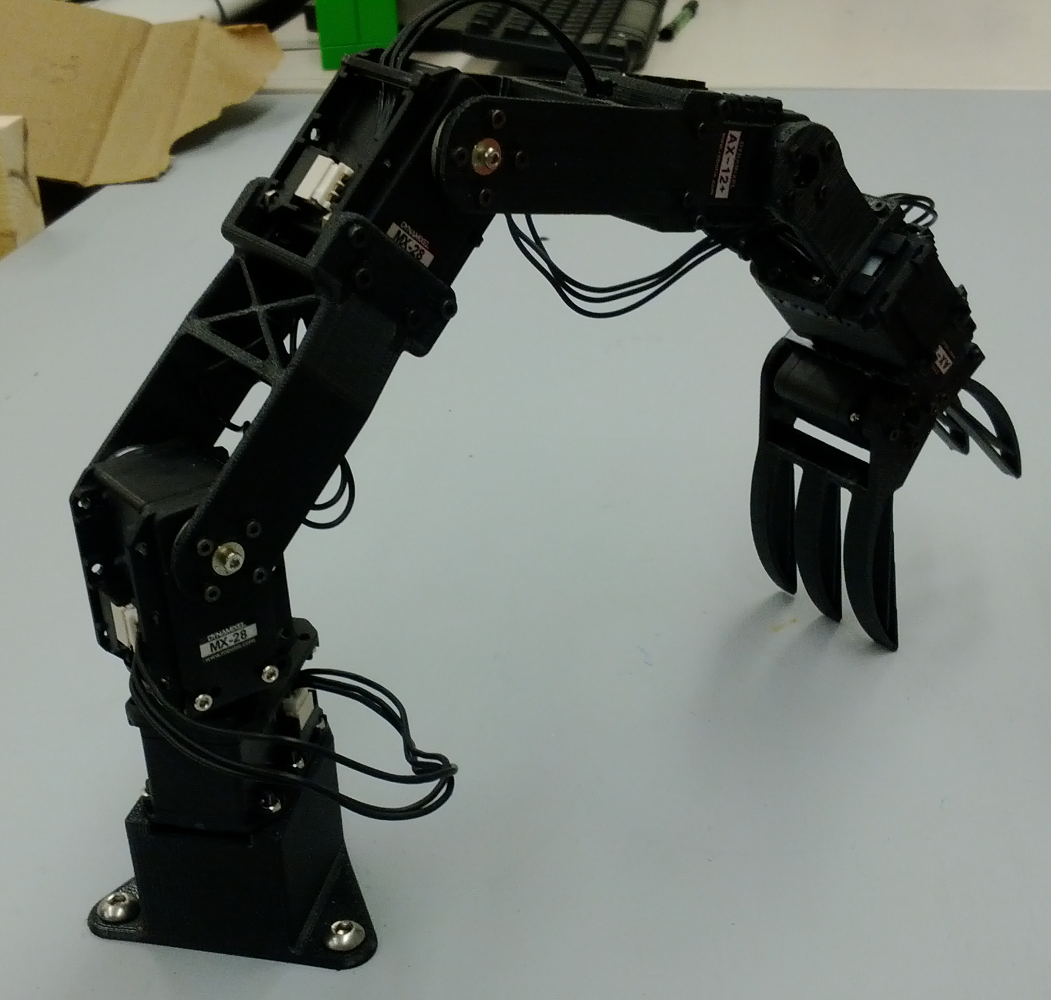
\includegraphics[height=3in]{figures/arm2.png}
    \label{fig:arm}
}
\subfloat[Kinect mount \xxx{placeholder}] {
    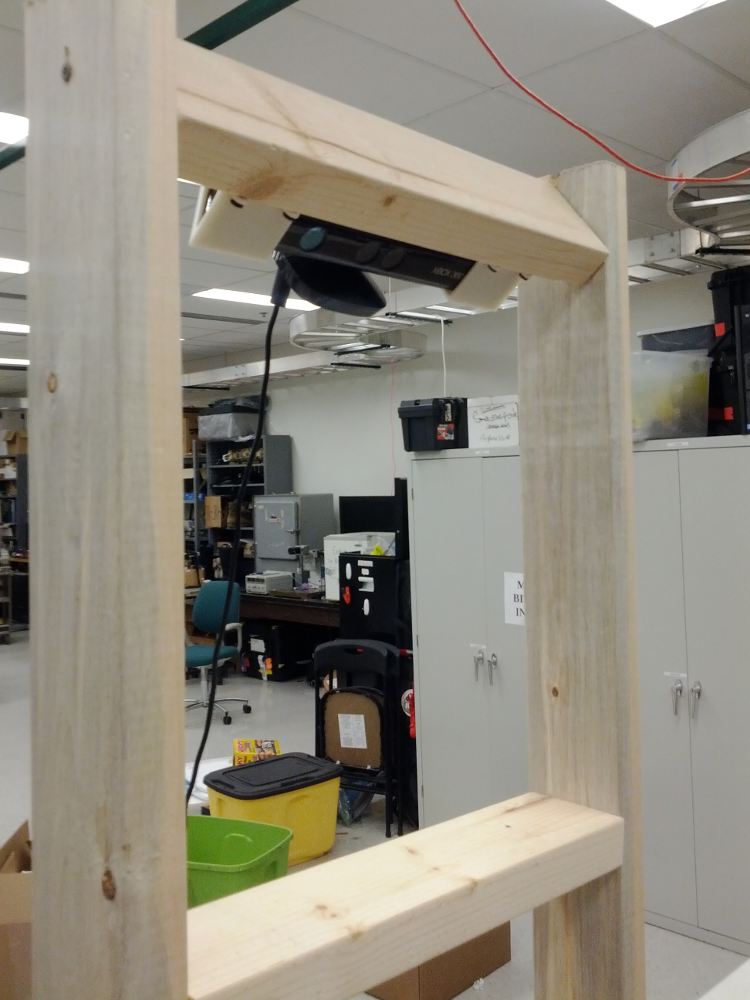
\includegraphics[height=3in]{figures/kinect.png}
    \label{fig:kinect-mount}
}
\caption{Our robotic arm and Kinect mount. \xxx{better caption}}
\label{fig:hardware}
\end{figure}

\subsection{Data Collection and Training}
We have acquired a large variety of children's foam blocks in many shapes and
colors to act as our objects for classification. A small subset of the blocks
can be seen in Figure~\ref{fig:blocks}. The foam the blocks is an ideal
material to work with as it
\begin{inparaenum}[(1)]
\item has a smooth, matte finish,
\item comes in a variety of distinct colors, and
\item is deformable enough to be grabbed by the arm but still retain its
shape.
\end{inparaenum}

We have collected a training dataset of footage of the foam blocks at numerous
positions and angles throughout the play area and are creating \xxx{have
created?} a tool that segments out objects from the scene and allows a human
to label these objects with relevant descriptors.

\xxx{More to come?}

\begin{figure}
\centering
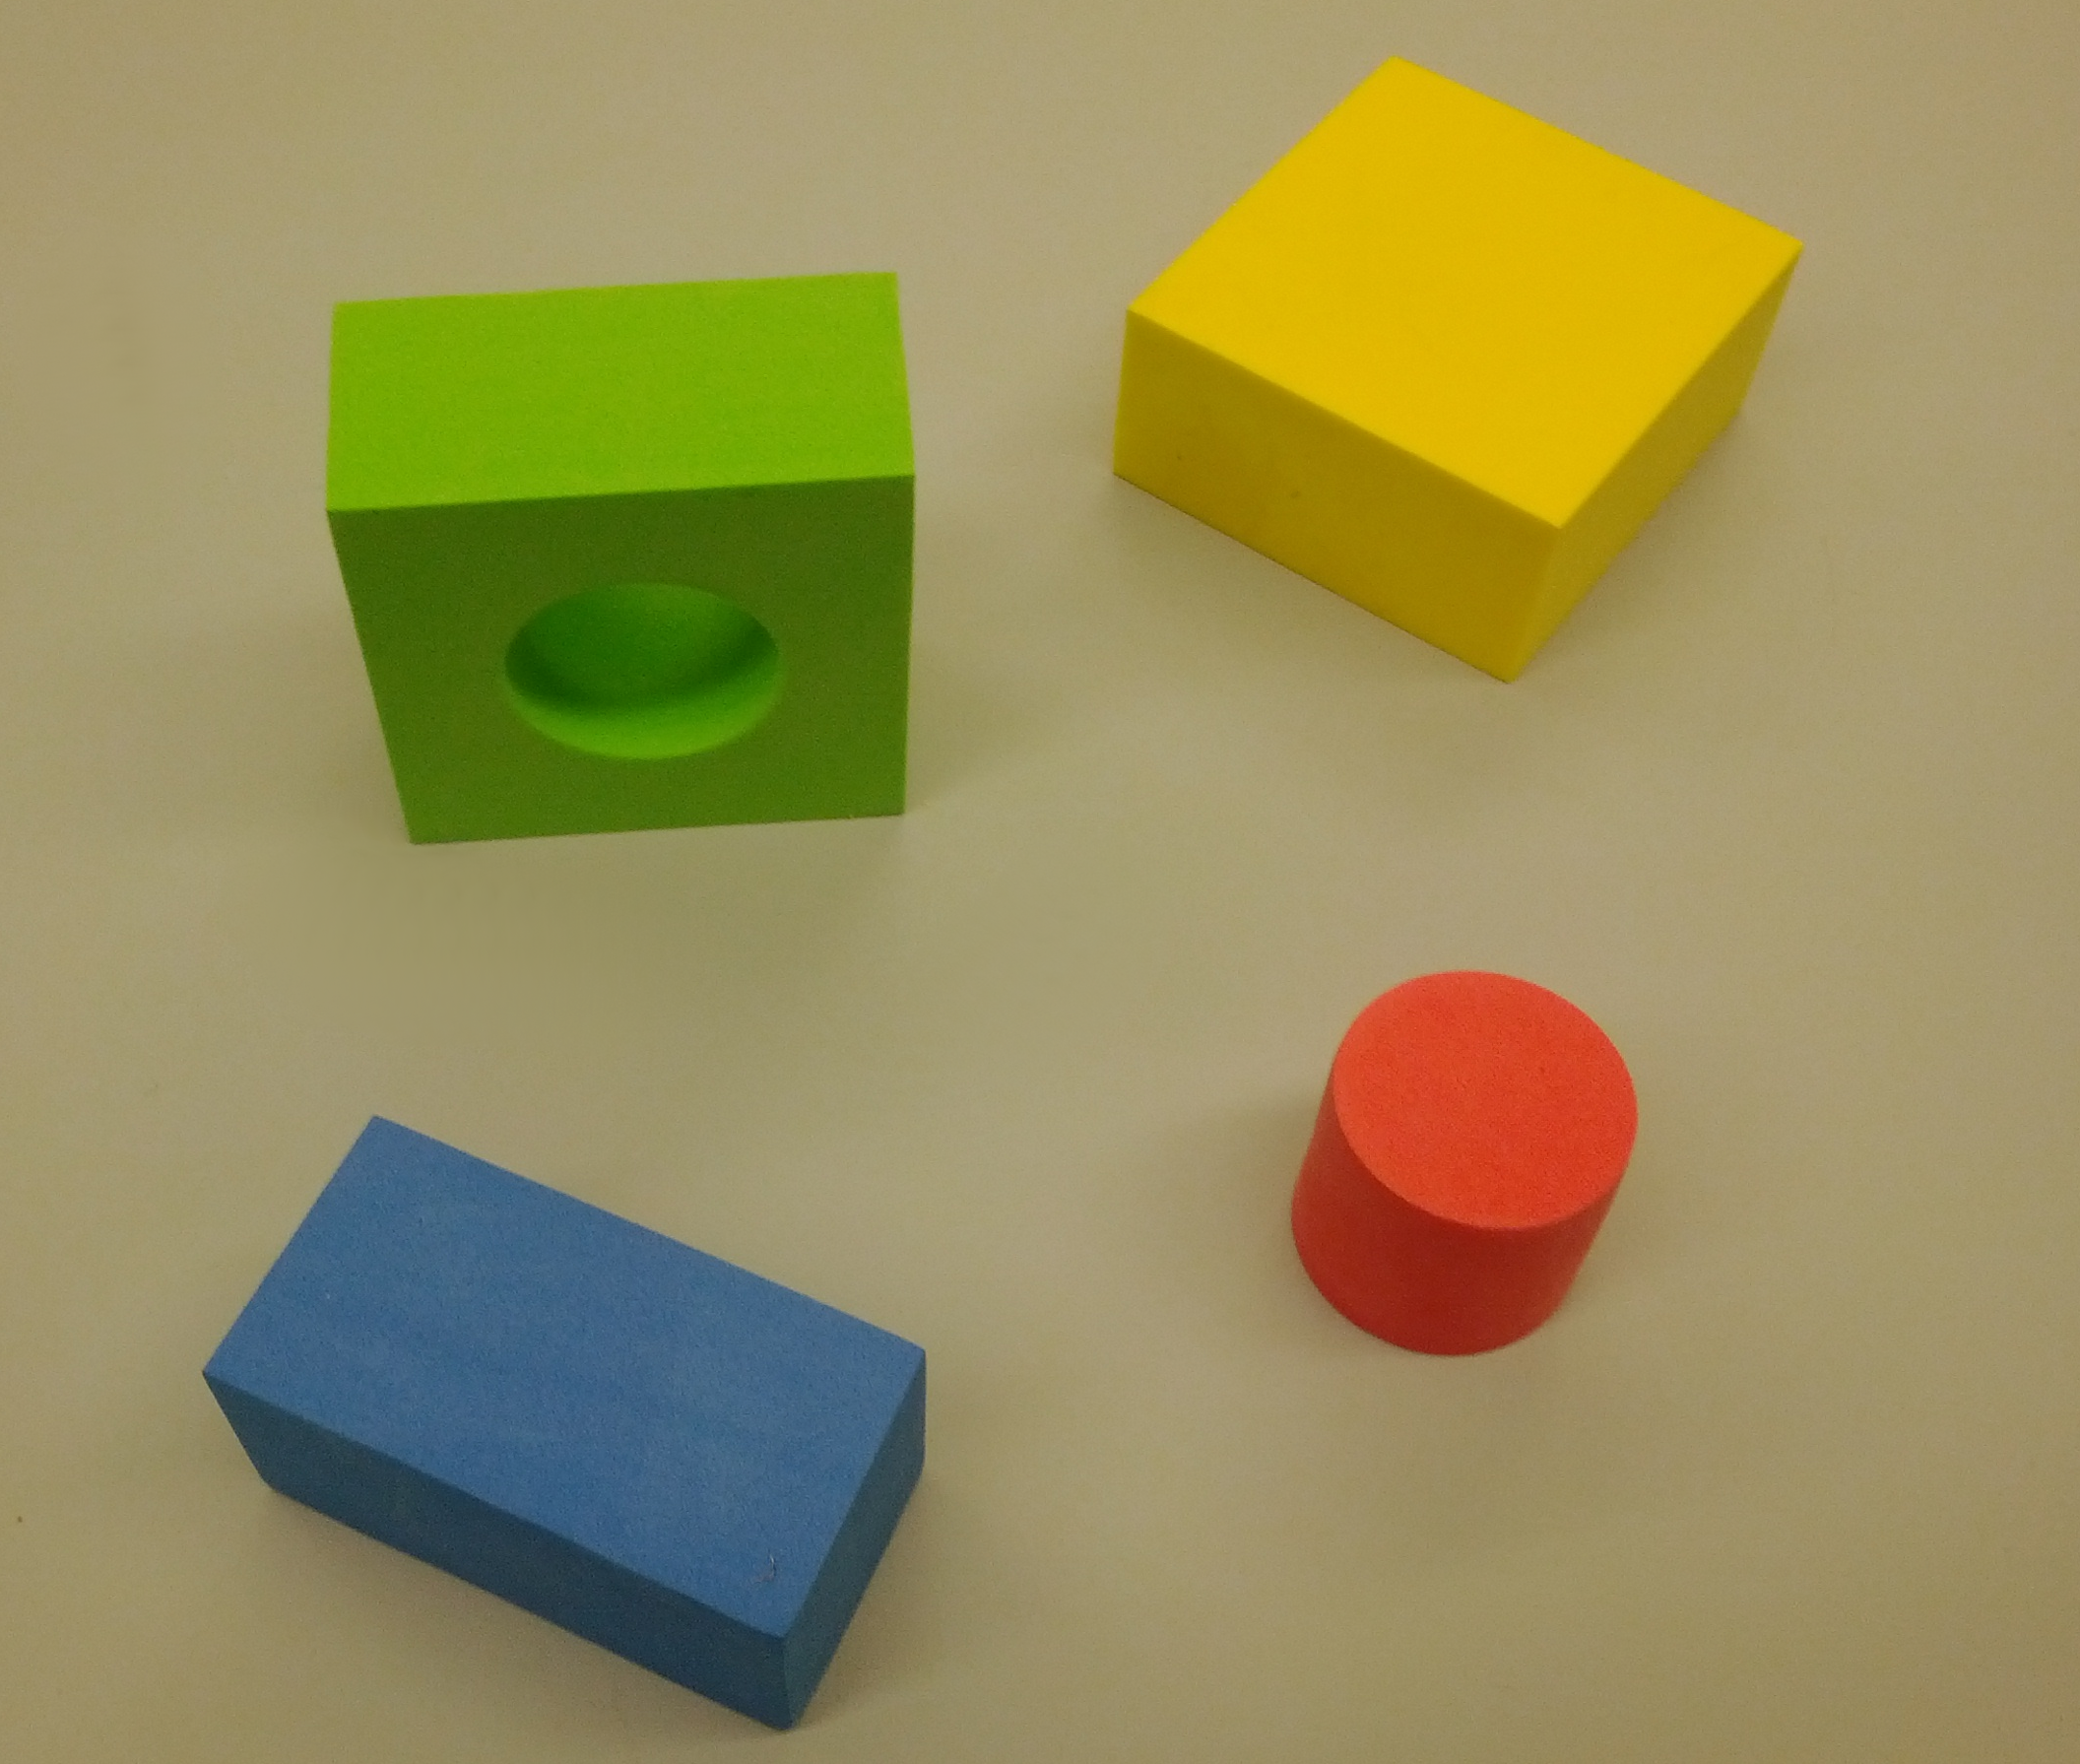
\includegraphics[width=0.48\textwidth]{figures/blocks.png}
\caption{A sample of the foam blocks we are using for classification. To
    simplify the language space we are working in, we limited our objects to
    those that can be described with simple shapes and colors.}
\label{fig:blocks}
\end{figure}

\section{Future Milestones}
\xxx{Dates and sub-goals (please set sub-goals on a weekly basis so that they
    can be done in a week)}

\meh{Due to a looming paper deadline on 10~Mar for Lauren and Rob, data
    processing for training purposes has taken a backseat to paper writing.
    Rapid progress is expected post-deadline when this additional workload
    disappears.}

\paragraph{11~Mar -- 17~Mar}

\paragraph{18~Mar -- 24~Mar}

\paragraph{25~Mar -- 31~Mar}

\paragraph{1~Apr -- 7~Apr}

\paragraph{8~Apr -- 14~Apr}

\paragraph{15~Apr -- 21~Apr}
\meh{
\begin{itemize}
    \item Begin written report
    \item Begin laying out poster
\end{itemize}

\paragraph{21~Apr -- 24~Apr}
\begin{itemize}
    \item Finish editing final report
    \item Finish editing poster and print final copy
\end{itemize}
}

\section{Conclusion}
\xxx{Summary of your progress and your final expected goal (what do you expect
    to achieve or demonstrate for the final project?)}

\bibliographystyle{plain}
\bibliography{literature}

\end{document}
